\section{Проектирование методики верификации}

В данном разделе рассматривается проектирование методики верификации
соответствия TLA+ спецификации и программной реализации. Сначала описывается
общая схема методики, включающая инструментирование кода, сбор и агрегацию
локальных трасс, а также построение ограниченной спецификации для их проверки.
Затем задача валидации трасс связывается с математической постановкой,
сформулированной в исследовательской части, и интерпретируется как задача
проверки совместимости наблюдаемой трассы с допустимым поведением модели.

\subsection{Методика верификации}

Предлагаемая методика верификации основана на сопоставлении трасс исполнения
распределённой реализации с формальной спецификацией, написанной на языке TLA+.
Общая схема подхода представлена на рисунке~\ref{fig:arch}.

\begin{figure}
  \centering
  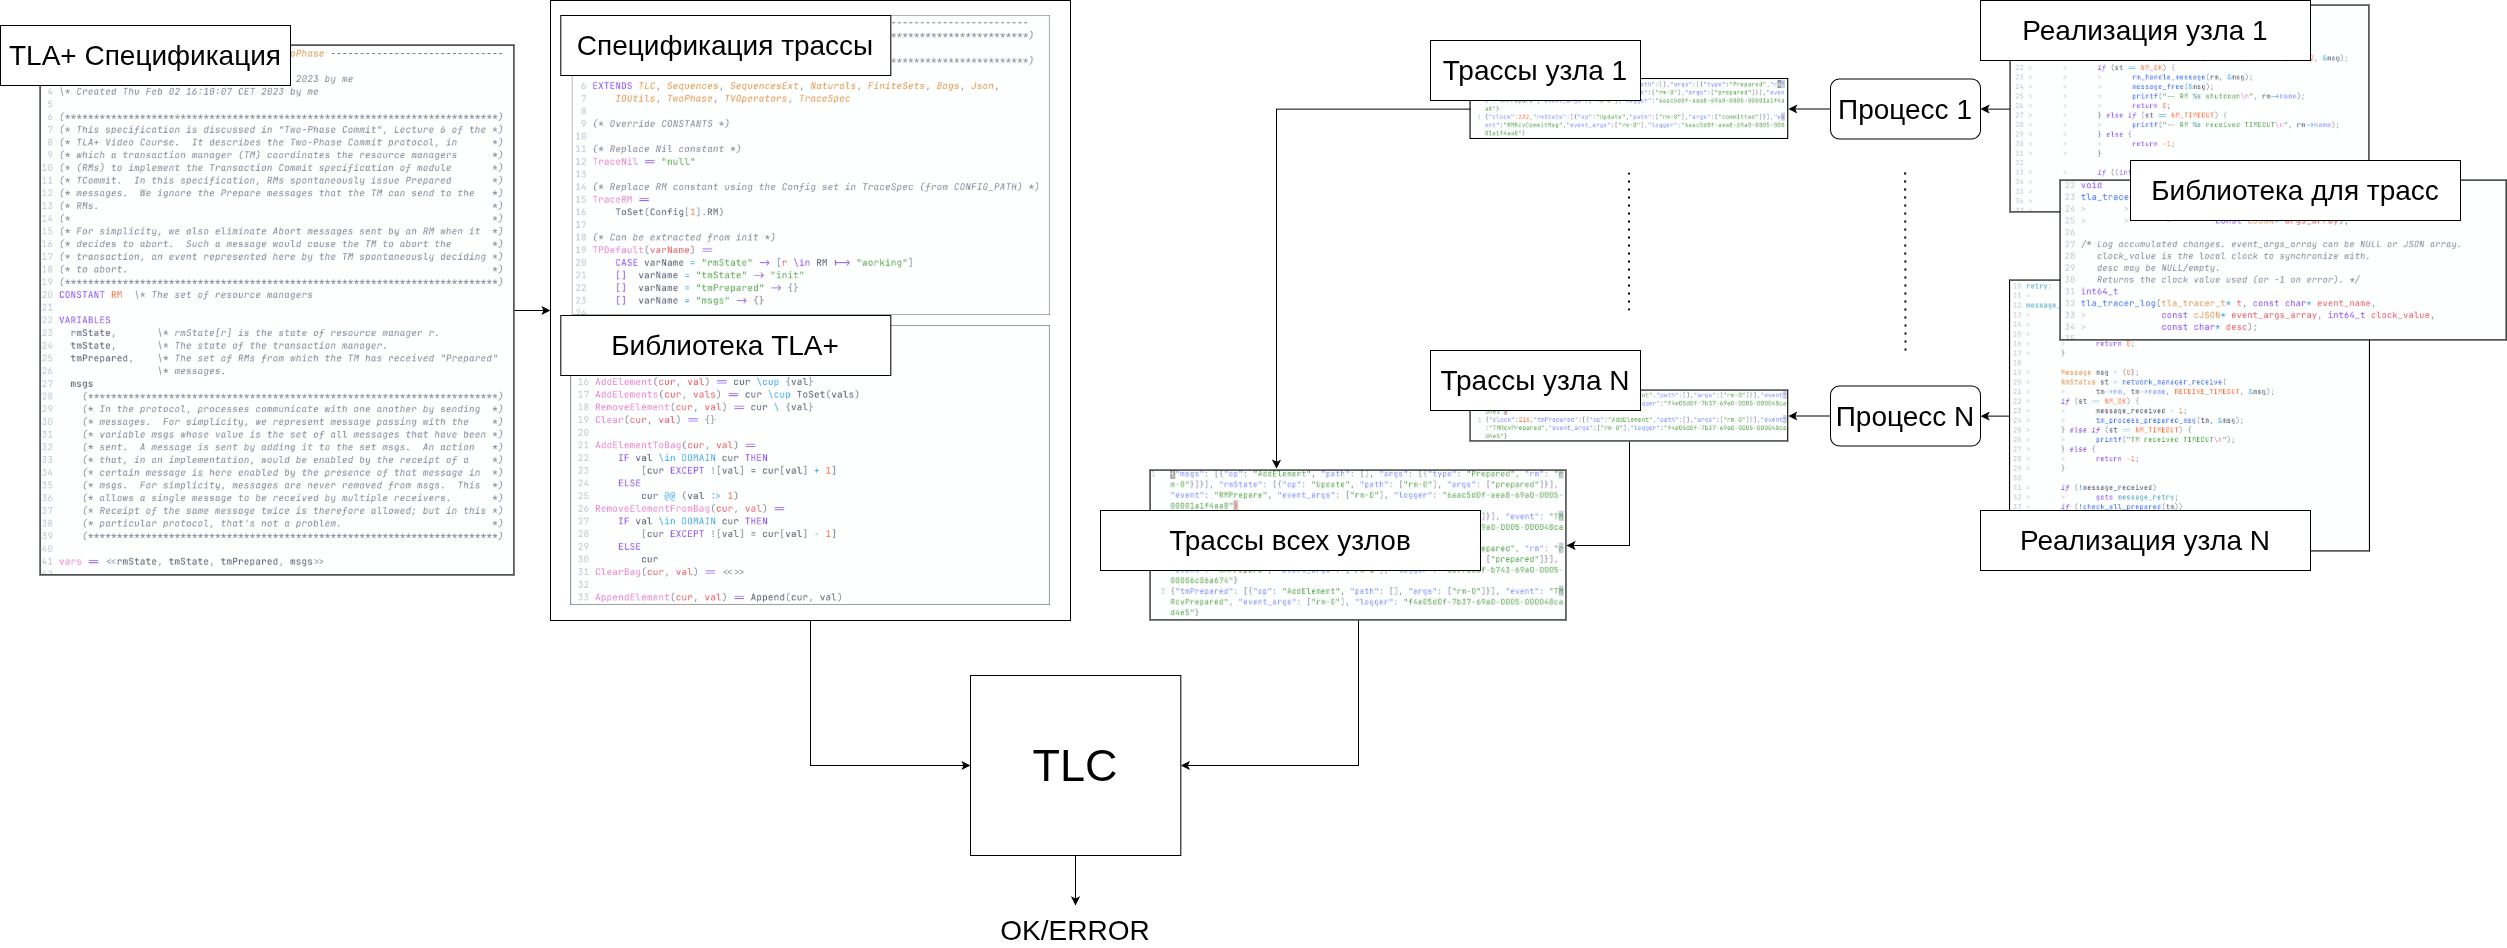
\includegraphics[scale=0.17]{inc/arch.png}
  \caption{Методика верификации}
  \label{fig:arch}
\end{figure}

Исходными артефактами являются:

\begin{itemize}
    \item программная реализация алгоритма;
    \item формальная спецификация этого алгоритма на языке TLA+.
\end{itemize}

Спецификация задаёт множество допустимых состояний системы и переходов между
ними, однако не содержит сведений о конкретной реализации. Реализация, в свою
очередь, выполняется в распределённой среде, где возможны различные порядки
доставки сообщений и недетерминированные сценарии выполнения.

Для сопоставления поведения реализации со спецификацией используется
инструментирование кода. В реализацию внедряется библиотека трассировки,
которая фиксирует события, соответствующие переходам спецификации, а также
изменения переменных спецификации. При выполнении системы каждый процесс
формирует собственную трассу в формате JSON, содержащую последовательность
операций обновления логических переменных модели.

Полученные локальные трассы агрегируются в единый глобальный файл, отражающий
наблюдаемую последовательность изменений состояния всей распределённой системы.
Таким образом, формируется абстрактное представление исполнения, выраженное в
терминах переменных TLA+, а не в терминах низкоуровневых операций кода.

Для проверки корректности трассы используется дополнительная спецификация
(\textit{Trace Specification}), построенная на основе исходной TLA+
спецификации. Она расширяет её таким образом, чтобы поведение модели было
ограничено наблюдаемой последовательностью изменений. Иными словами, трасса
интерпретируется как частичное ограничение на допустимые переходы модели.

Далее средство модельной проверки TLC используется для проверки существования
поведения спецификации, согласованного с данной трассой. Если TLC подтверждает
корректность, это означает, что наблюдаемое исполнение допустимо спецификацией.
В противном случае обнаруживается расхождение между реализацией и моделью, и
TLC предоставляет контрпример, позволяющий локализовать проблему.

\subsection{Задача валидации трасс}

В терминах математической постановки, введённой в исследовательской части,
спецификация рассматривается как система переходов $\mathcal{M} = (X, X_0, R)$,
где $X$ --- множество состояний, $X_0$ --- множество начальных состояний, а $R$
--- отношение допустимых переходов. Наблюдаемая трасса программы задаётся
последовательностью $\tau = (\sigma_1,\sigma_2,\dots,\sigma_m)$, а соответствие
между элементом трассы и переходом модели задаётся предикатом согласованности
$C : \Sigma \times X \times X \to \{0,1\}$.

Тогда задача валидации трассы сводится к проверке, существует ли такое конечное
поведение модели, которое одновременно допускается спецификацией и согласуется
со всей наблюдаемой трассой. Введённые ранее множества
$\mathrm{B}_m(\mathcal{M})$ и $\mathrm{M}_m(\tau)$ позволяют записать это
условие в виде
\[
\mathrm{B}_m(\mathcal{M}) \cap \mathrm{M}_m(\tau) \neq \varnothing.
\]
Именно это условие выражает полную совместимость трассы с моделью.

Иначе говоря, требуется установить, существует ли путь в графе состояний
спецификации, который начинается в одном из допустимых начальных состояний и
может быть сопоставлен всей последовательности наблюдений трассы. В более общем
виде задача формулируется как нахождение максимального согласованного префикса
трассы, то есть величины
\[
k^*(\mathcal{M},\tau)
=
\max K_{\mathrm{доп}}(\mathcal{M},\tau),
\]
где $K_{\mathrm{доп}}(\mathcal{M},\tau)$ --- множество длин
префиксов трассы, совместимых с моделью. Если
$k^*(\mathcal{M},\tau)=m$, то вся трасса согласована со
спецификацией; если же $k^*(\mathcal{M},\tau)<m$, то расхождение
между реализацией и моделью возникает начиная с позиции
$k^*(\mathcal{M},\tau)+1$.

Рис.~\ref{fig:traces-search} иллюстрирует данную идею. Слева изображается
линейная цепочка наблюдений, соответствующая трассе, полученной из
инструментированной реализации. Справа представлен граф состояний, определяемый
спецификацией TLA+. Проверка заключается в поиске пути в графе состояний
спецификации, который можно сопоставить данной трассе.

\begin{figure}
  \centering
  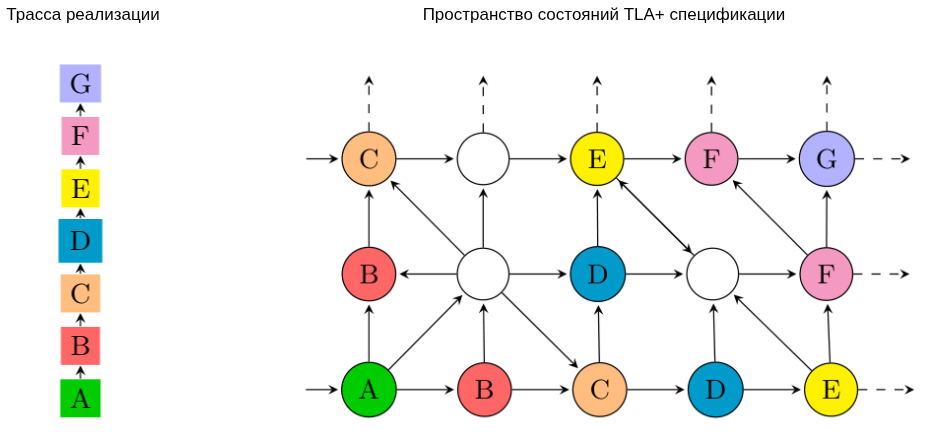
\includegraphics[scale=0.5]{inc/traces-search.png}
  \caption{Валидация трассы как поиск пути в пространстве состояний}
  \label{fig:traces-search}
\end{figure}

Первое состояние искомого поведения должно принадлежать множеству $X_0$. Далее
для каждого следующего элемента трассы необходимо найти по крайней мере один
допустимый переход модели, согласованный с данным наблюдением. Поскольку трасса
обычно содержит неполную информацию о состоянии, одному и тому же наблюдению
может соответствовать несколько переходов модели. Если для некоторого префикса
трассы не существует ни одного допустимого продолжения, согласованного со
следующим наблюдением, соответствующая ветвь поиска отбрасывается.

Следует учитывать, что атомарные шаги реализации не всегда в точности совпадают
с атомарными переходами спецификации. Поэтому на уровне проектируемой методики
предполагается, что необходимое согласование гранулярности выполняется при
построении трассы и ограниченной спецификации: несколько низкоуровневых
действий реализации могут быть объединены в один логический шаг,
соответствующий одному переходу модели, либо, наоборот, один шаг реализации
может интерпретироваться через композицию действий спецификации. После такого
приведения задача вновь сводится к проверке совместимости трассы с моделью в
смысле приведённой выше математической постановки.

Практически эта редукция реализуется с помощью дополнительной спецификации
трассы и модельного проверяющего TLC. В общем случае разработчик должен явно
задать соответствие между именами событий в трассе и действиями спецификации, а
также между именами логируемых переменных и переменными TLA+. Тем самым задача
валидации трасс становится конструктивным воплощением ранее сформулированной
математической постановки задачи верификации соответствия спецификации и
реализации.
